\documentclass{article}
\usepackage{pgfplots}
\pgfplotsset{compat=1.18}

\begin{document}

\begin{figure}[ht]
    \centering
    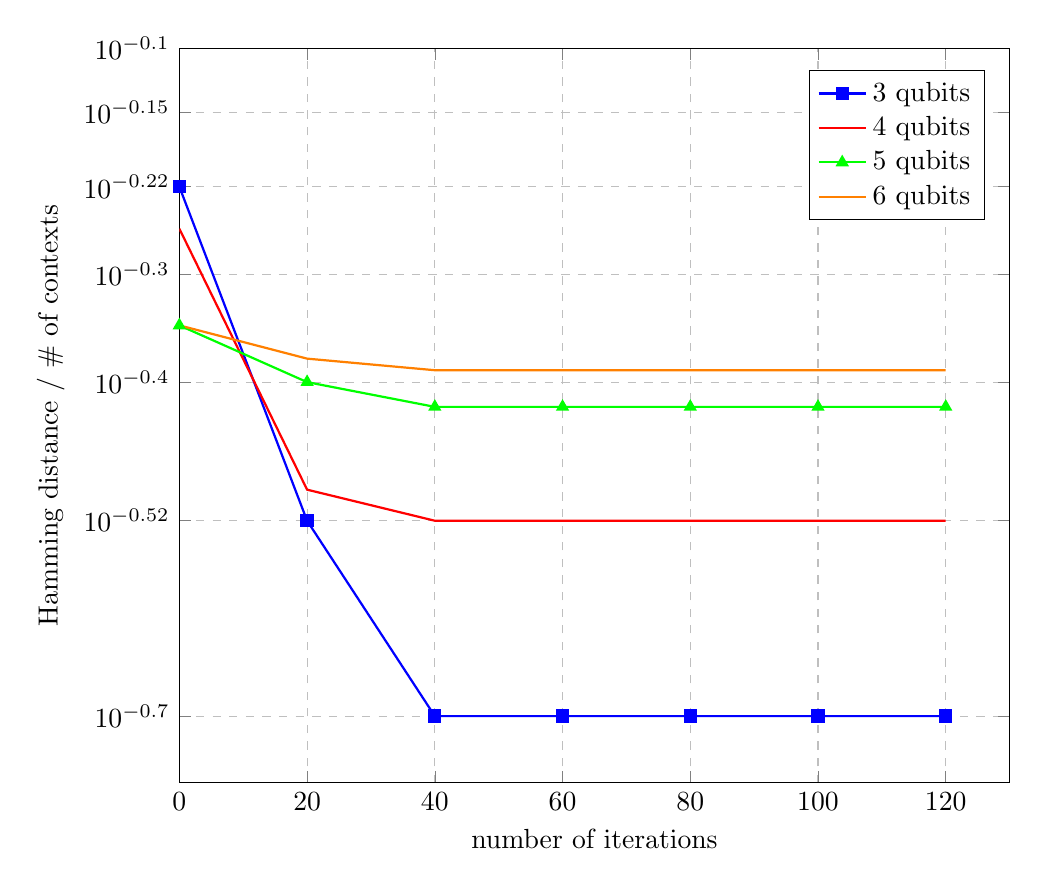
\begin{tikzpicture}
        \begin{semilogyaxis}[
            xlabel={number of iterations},
            ylabel={Hamming distance / \# of contexts},
            xmin=0, xmax=130,
            ymin=0, ymax=0.8,
            xtick={0, 20, 40, 60, 80, 100, 120},
            ytick={0.0, 0.1, 0.2, 0.3, 0.4, 0.5, 0.6, 0.7, 0.8},
            legend pos=north east,
            grid=major,
            grid style=dashed,
            title style={at={(0.5,1.05)}, anchor=south},
            title={},
            height=0.9\textwidth,
            width=\textwidth,
            every axis plot/.append style={
                mark options={solid},
                mark size=2pt,
                mark options={solid}
            }
        ]
            \addplot[blue, mark=square*, thick] coordinates {
                (0, 0.6)
                (20, 0.3)
                (40, 0.2)
                (60, 0.2)
                (80, 0.2)
                (100, 0.2)
                (120, 0.2)
            };
            \addplot[red, mark=o*, thick] coordinates {
                (0, 0.55)
                (20, 0.32)
                (40, 0.3)
                (60, 0.3)
                (80, 0.3)
                (100, 0.3)
                (120, 0.3)
            };
            \addplot[green, mark=triangle*, thick] coordinates {
                (0, 0.45)
                (20, 0.4)
                (40, 0.38)
                (60, 0.38)
                (80, 0.38)
                (100, 0.38)
                (120, 0.38)
            };
            \addplot[orange, mark=x*, thick] coordinates {
                (0, 0.45)
                (20, 0.42)
                (40, 0.41)
                (60, 0.41)
                (80, 0.41)
                (100, 0.41)
                (120, 0.41)
            };
            
            \legend{3 qubits, 4 qubits, 5 qubits, 6 qubits}
        \end{semilogyaxis}
    \end{tikzpicture}
    \caption{Minimal Hamming distances (the \(y\)-axis) per total number of contexts, over the number of iterations (the \(x\)-axis), computed by the heuristic method running simultaneously on 200 threads shared between 20 cores of an Intel(R) Core(TM) i7-12700H processor, for the quantum configurations composed of all the lines of the three- to six-qubit symplectic polar spaces.}
    \label{fig:minimal_hamming_distances}
\end{figure}

\end{document}